\section{Describing flexibility from TCLs}\label{sec:monetizing_flex}

There are several ways to monetize flexibility from TCLs. In this section, we focus on mFRR and load shifting. First, we describe how to mathematically model a TCL as a flexible resource. Second, we describe how to monetize the flexibility from TCLs for mFRR and load shifting, and provide the objective functions in both cases. For mFRR, the objective function includes all costs and revenues for the BRP, while for load shifting, the objective function only includes the flexible demand's perspective. This approach explicitly shows the situation where flexible demand is activated without including the BRP, as this is more realistic.

\subsection{Modelling TCL as a flexible resource}

TCLs are characterized by being controlled such that the temperature is kept at a specified setpoint. Examples include heat pumps, freezers, air condition units, ovens, etc. They are widely believed to constitute an important part of demand-side flexibility due to the inherent thermal inertia of such temperature-driven systems \cite{hao2014aggregate}.

In this paper, we focus on freezers, which are a very common type of TCLs. Specifically, we focus on a single freezer display in a Danish supermarket. Freezers are characterized by a large thermal inertia due to the frozen food, which makes them suitable for flexibility. On the other hand, there is a risk of food degradation when utilizing flexibility. Therefore, it is important to model the temperature dynamics in the freezer for a realistic and risk-aware estimation of its flexibility.

The rest of the section is organized as follows. First, we visualize the measurements from a real supermarket freezer. Second, we introduce a second-order grey-box model that characterizes the supermarket freezer. Third, we validate the second-order model and show how it can be used to simulate demand response from a freezer.

\subsubsection{Supermarket freezer description}

%In this paper, data from a single freezer operating in a large Danish supermarket is used as a case study. In Figure \ref{fig:chunk}, the air temperature and opening degree of the freezer is shown together with the electric power of the variable-speed compressor rack for a single day. All values correspond to 15-min averages. Temperature fluctuates around its setpoint at -18 $^{\circ}$C with the exception of hour 7-8, where defrosting is scheduled. While defrosting, a heating element is briefly turned on, and the expansion valve is closed such that the flow of refrigerant stops. Afterwards, while recovering the temperature, the expansion valve is fully opened. The power consumption of the compressor rack, scaled to one freezer, is shown in the bottom plot. Power consumption is highest during opening hours, and it is lowest during closing hours. During opening hours, food is being replaced and customers open the display case constantly. Furthermore, most supermarkets put additional insulation on the display cases during closing hours which reduces thermal losses. For these reasons, there are effectively two regimes for a supermarket freezer plus a short defrosting regime.

In this paper, data from a single freezer operating in a large Danish supermarket is used as a case study.
In Figure \ref{fig:chunk}, the top plot shows 15-min average air temperature of the freezer, while the middle plot shows the opening degree of the valve.
Temperature fluctuates around its setpoint at -18 $^{\circ}$C with the exception of hour 7-8, where defrosting is scheduled.
While defrosting, a heating element is briefly turned on, and the expansion valve is closed such that the flow of refrigerant stops. Afterwards, while recovering the temperature, the expansion valve is fully opened.
The electric power of the variable-speed compressor rack, scaled to one freezer\footnote{Since temperature dynamics are similar for all freezers, homogeneity is assumed. Hence, equal consumption is assumed for all freezers.}, is shown in the bottom plot.
Consumption is highest during opening hours, and it is lowest during closing hours.
During opening hours, food is being replaced and customers open the display case constantly.
Furthermore, most supermarkets put additional insulation on the display cases during closing hours which reduces thermal losses.
For these reasons, there are effectively two regimes for a supermarket freezer plus a short defrosting regime.
\begin{figure}[!t]
    \centering
    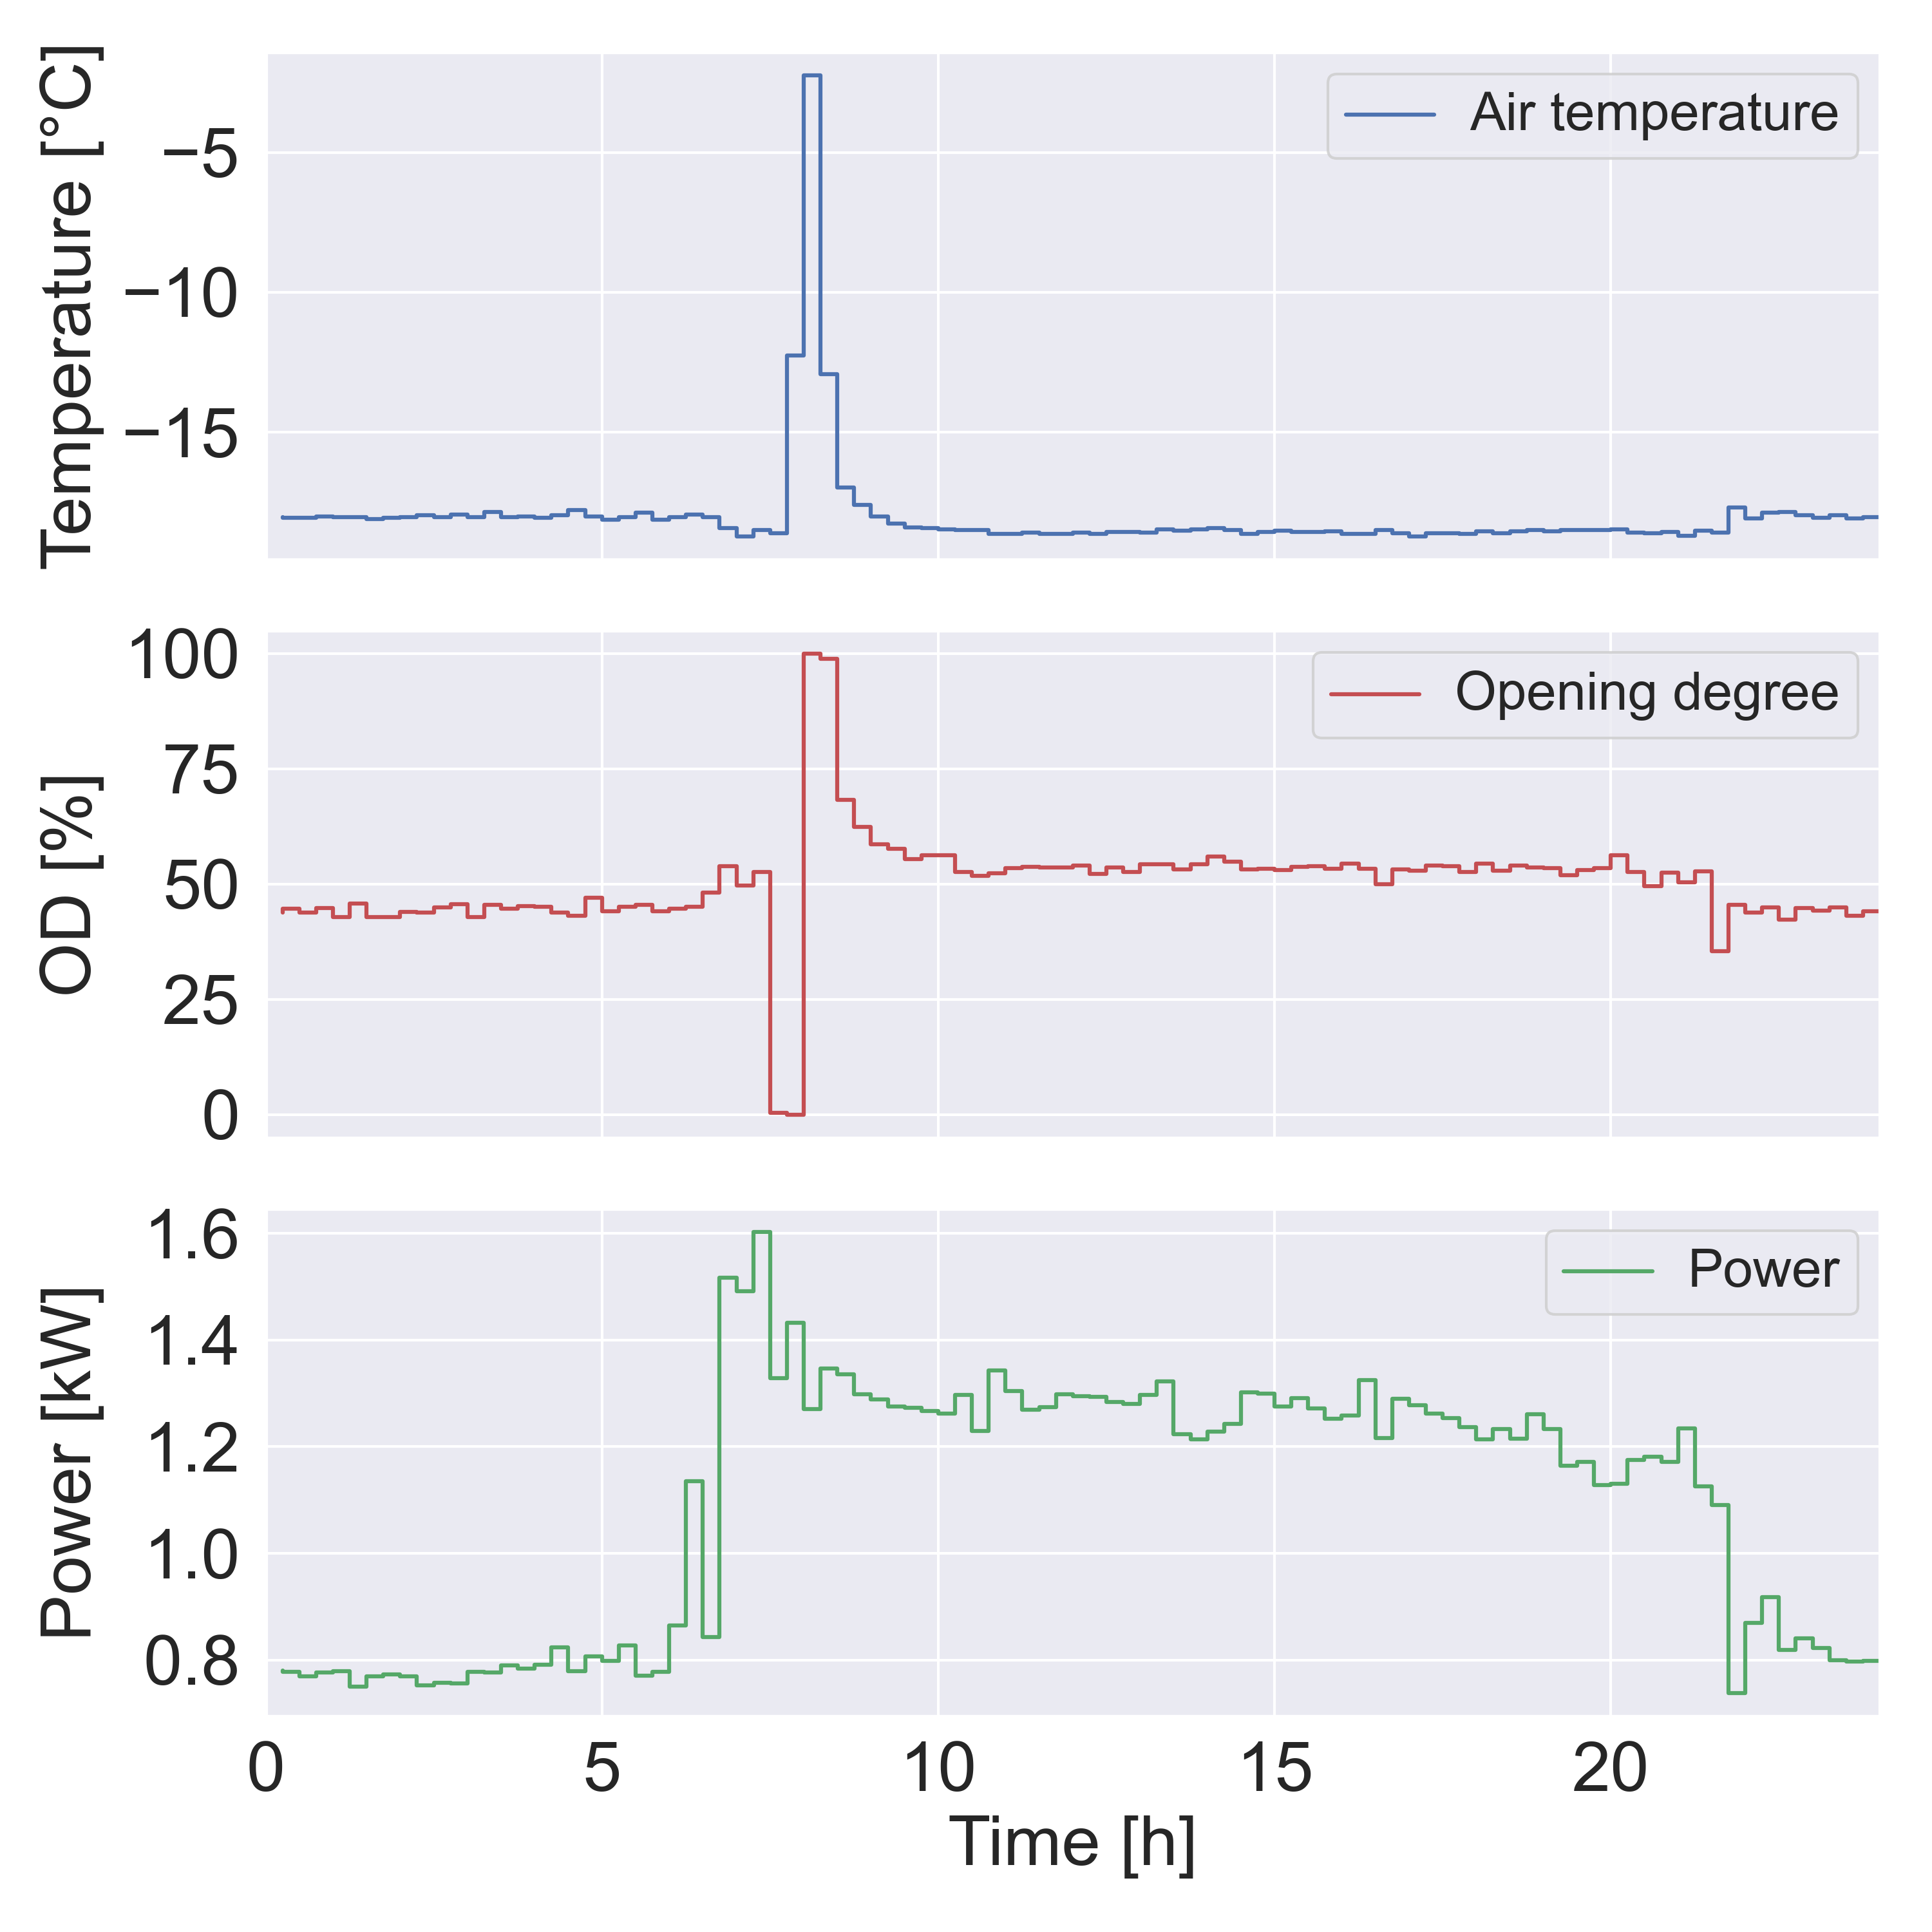
\includegraphics[width=\columnwidth]{../figures/tmp_od_Pt.png}
    \caption{\textbf{Top}: temperature of a single freezer in a supermarket. \textbf{Middle}: opening degree of the freezer expansion valve. \textbf{Bottom}: power of the compressor rack feeding a single freezer.}
    \label{fig:chunk}
\end{figure}

\subsubsection{Thermal modelling of freezer}

In \cite{hao2014aggregate}, it is described how a simple TCL model can be made. We extend it to a second-order state-space model that accounts for the thermal mass of the food, which essentially provides the flexibility in freezers:

\begin{subequations}\label{eq:2ndFreezerStateSpace}
    \begin{align}
        T^{f}_{t+1} & = T^{f}_{t} + dt \cdot \frac{1}{C^f}\left(\frac{1}{R^{cf}} (T^{c}_{t} - T^{f}_{t}) \right)                                                                              \\
        T^{c}_{t+1} & = T^{c}_t + dt \cdot \frac{1}{C^c}\Bigl(\frac{1}{R^{cf}} (T^{f}_t - T^{c}_t) + \frac{1}{R^{ci}_{t}} (T^{i}_t - T^{c}_t)                                          \notag \\ & \mspace{50mu} - \eta \cdot OD_t P_t \Bigr) + \epsilon \mathbbm{1}^{\text{df}}_{t}
    \end{align}
\end{subequations}

Here, $T^c$ is the air temperature in the freezer which is measured, and $T^f$ is the food temperature which is a latent, unobserved state. It is essentially a low-pass filter of the air temperature in the freezer with time constant $\tau = C^f R^{cf}$. $C^f$ and $C^c$ are the thermal capacitance of the food and air in the freezer, respectively. $R^{cf}$ and $R^{ci}$ are the thermal resistance between food and air in the freezer, and air and indoor temperature, respectively. Furthermore, $\epsilon$ represents the temperature change when defrosting and $\mathbbm{1}^{\textbf{df}}_{t}$ is the indicator function for when defrosting happens. $R^{ci}$ is either one of two values, $R^{ci, \text{day}}$ and $R^{ci, \text{night}}$, to capture the differences between opening hours (6 am to 10 pm) and closing hours (10 pm to 6 am). The opening degree, $OD_t$, and power $P_t$, are exogenous inputs as the opening degree is assumed to be fixed during a demand-response event, while only $P_t$ is controllable. $\eta$ is the compressor efficiency which resembles the coefficient of performance (COP). The model is discretized with a time step of 15 minutes, i.e. $dt = 0.25$ hours.

\subsubsection{Model validation}

Using the R library CTSM-R \cite{juhl2016ctsmr}, the parameters in (\ref{eq:2ndFreezerStateSpace}) have been estimated as shown in Table \ref{tab:parameter_estimates}. Notice that the thermal capacitance of the air in the freezer is significantly smaller than the thermal capacitance of the food, indicating that that the food temperature changes comparatively slower. The thermal resistance between the food and air inside the freezer, $R^{cf}$, is also significantly smaller than the thermal resistance between the air in the freezer and the indoor temperature in the supermarket, $R^{ci}$, both during the day and night. This makes sense as the lid acts as a physical barrier insulating the freezer. Furthermore, the thermal resistance to the indoor air temperature is higher during the night, which means that less power is needed, as seen in Figure \ref{fig:chunk}.

\begin{table}[!t]
    \caption{Parameter Estimates of (\ref{eq:2ndFreezerStateSpace}).}
    \label{tab:parameter_estimates}
    \centering
    \begin{tabular}[b]{|l|l|l|}
        \hline
        Parameter              & Value & Unit            \\ \hhline{|=|=|=|}
        $C^f$                  & 6.552 & kWh/$^{\circ}$C \\
        $C^c$                  & 0.077 & kWh/$^{\circ}$C \\
        $R^{cf}$               & 5.010 & $^{\circ}$C/kW  \\
        $R^{ci, \text{day}}$   & 41.05 & $^{\circ}$C/kW  \\
        $R^{ci, \text{night}}$ & 61.25 & $^{\circ}$C/kW  \\
        $\eta$                 & 1.561 &                 \\
        $\epsilon$             & 3.372 & $^{\circ}$C/h   \\ \hline
    \end{tabular}
\end{table}


The one-step residuals for the air temperature should ideally resemble white noise in order for a model to capture all dynamics seen in the data \cite{madsen2007time}. Figure \ref{fig:2ndFreezerModelValidation} shows the auto-correlation and cumulative periodogram of the residuals. The autocorrelation shows two significant lags for lag two and seven, but looks good otherwise. Likewise, in the periodogram it seems the model is able to capture most dynamics at all frequencies.

\begin{figure}[!t]
    \centering
    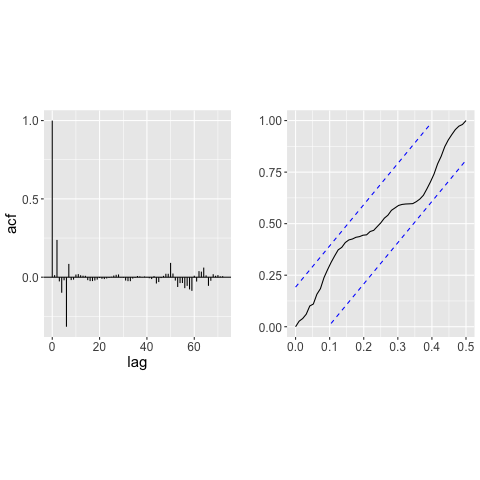
\includegraphics[width=\columnwidth]{../figures/2ndFreezerModelValidation.png}
    \caption{ Validation of the state-space model in (\ref{eq:2ndFreezerStateSpace}). \textbf{Left}: auto-correlation function of the model residuals. \textbf{Right}: cumulated periodogram of the residuals.}
    \label{fig:2ndFreezerModelValidation}
\end{figure}

Since there are only 96 time-steps, the defrosting period can result in relatively large residuals as it is difficult to capture such fast, transient dynamics. Since up-regulation is not allowed during defrosting, the residuals are not too important during that period. To decrease their effect in the parameter estimation procedure, the term $ \epsilon \mathbbm{1}^{\text{df}}_{t}$ was added to (\ref{eq:2ndFreezerStateSpace}) (see implementation details in code \cite{}).

Furthermore, Figure \ref{fig:2ndFreezerModelSimulation} (left) shows a 24-hour simulation of model (\ref{eq:2ndFreezerStateSpace}). It is seen that the simulation is very reasonable and closely follows the measured air temperature. Such a visual validation is important because the model will be embedded in an optimization model (cf. Section \ref{sec:OptimizationModel}).

It is also important to note that ideally the validation of (\ref{eq:2ndFreezerStateSpace}) would also include real measurements from the air and food temperature in a freezer during demand response events. However, by adhering to the fundamental physics governing the temperature dynamics as shown, the model is trusted to be accurate during demand response events too. It brings an intuitive interpretation which can be used to understand the impact on temperature during a demand response event.

In Figure \ref{fig:2ndFreezerModelSimulation} (right), such a simulated example of a demand response event is shown. It can clearly be seen how the air temperature increases when the power is turned off, and how it decreases when the power is turned back on. The food temperature is much more stable and only changes slightly, as expected. The rebound occurs until the food temperature is back to its normal value.

\begin{figure}[!t]
    \centering
    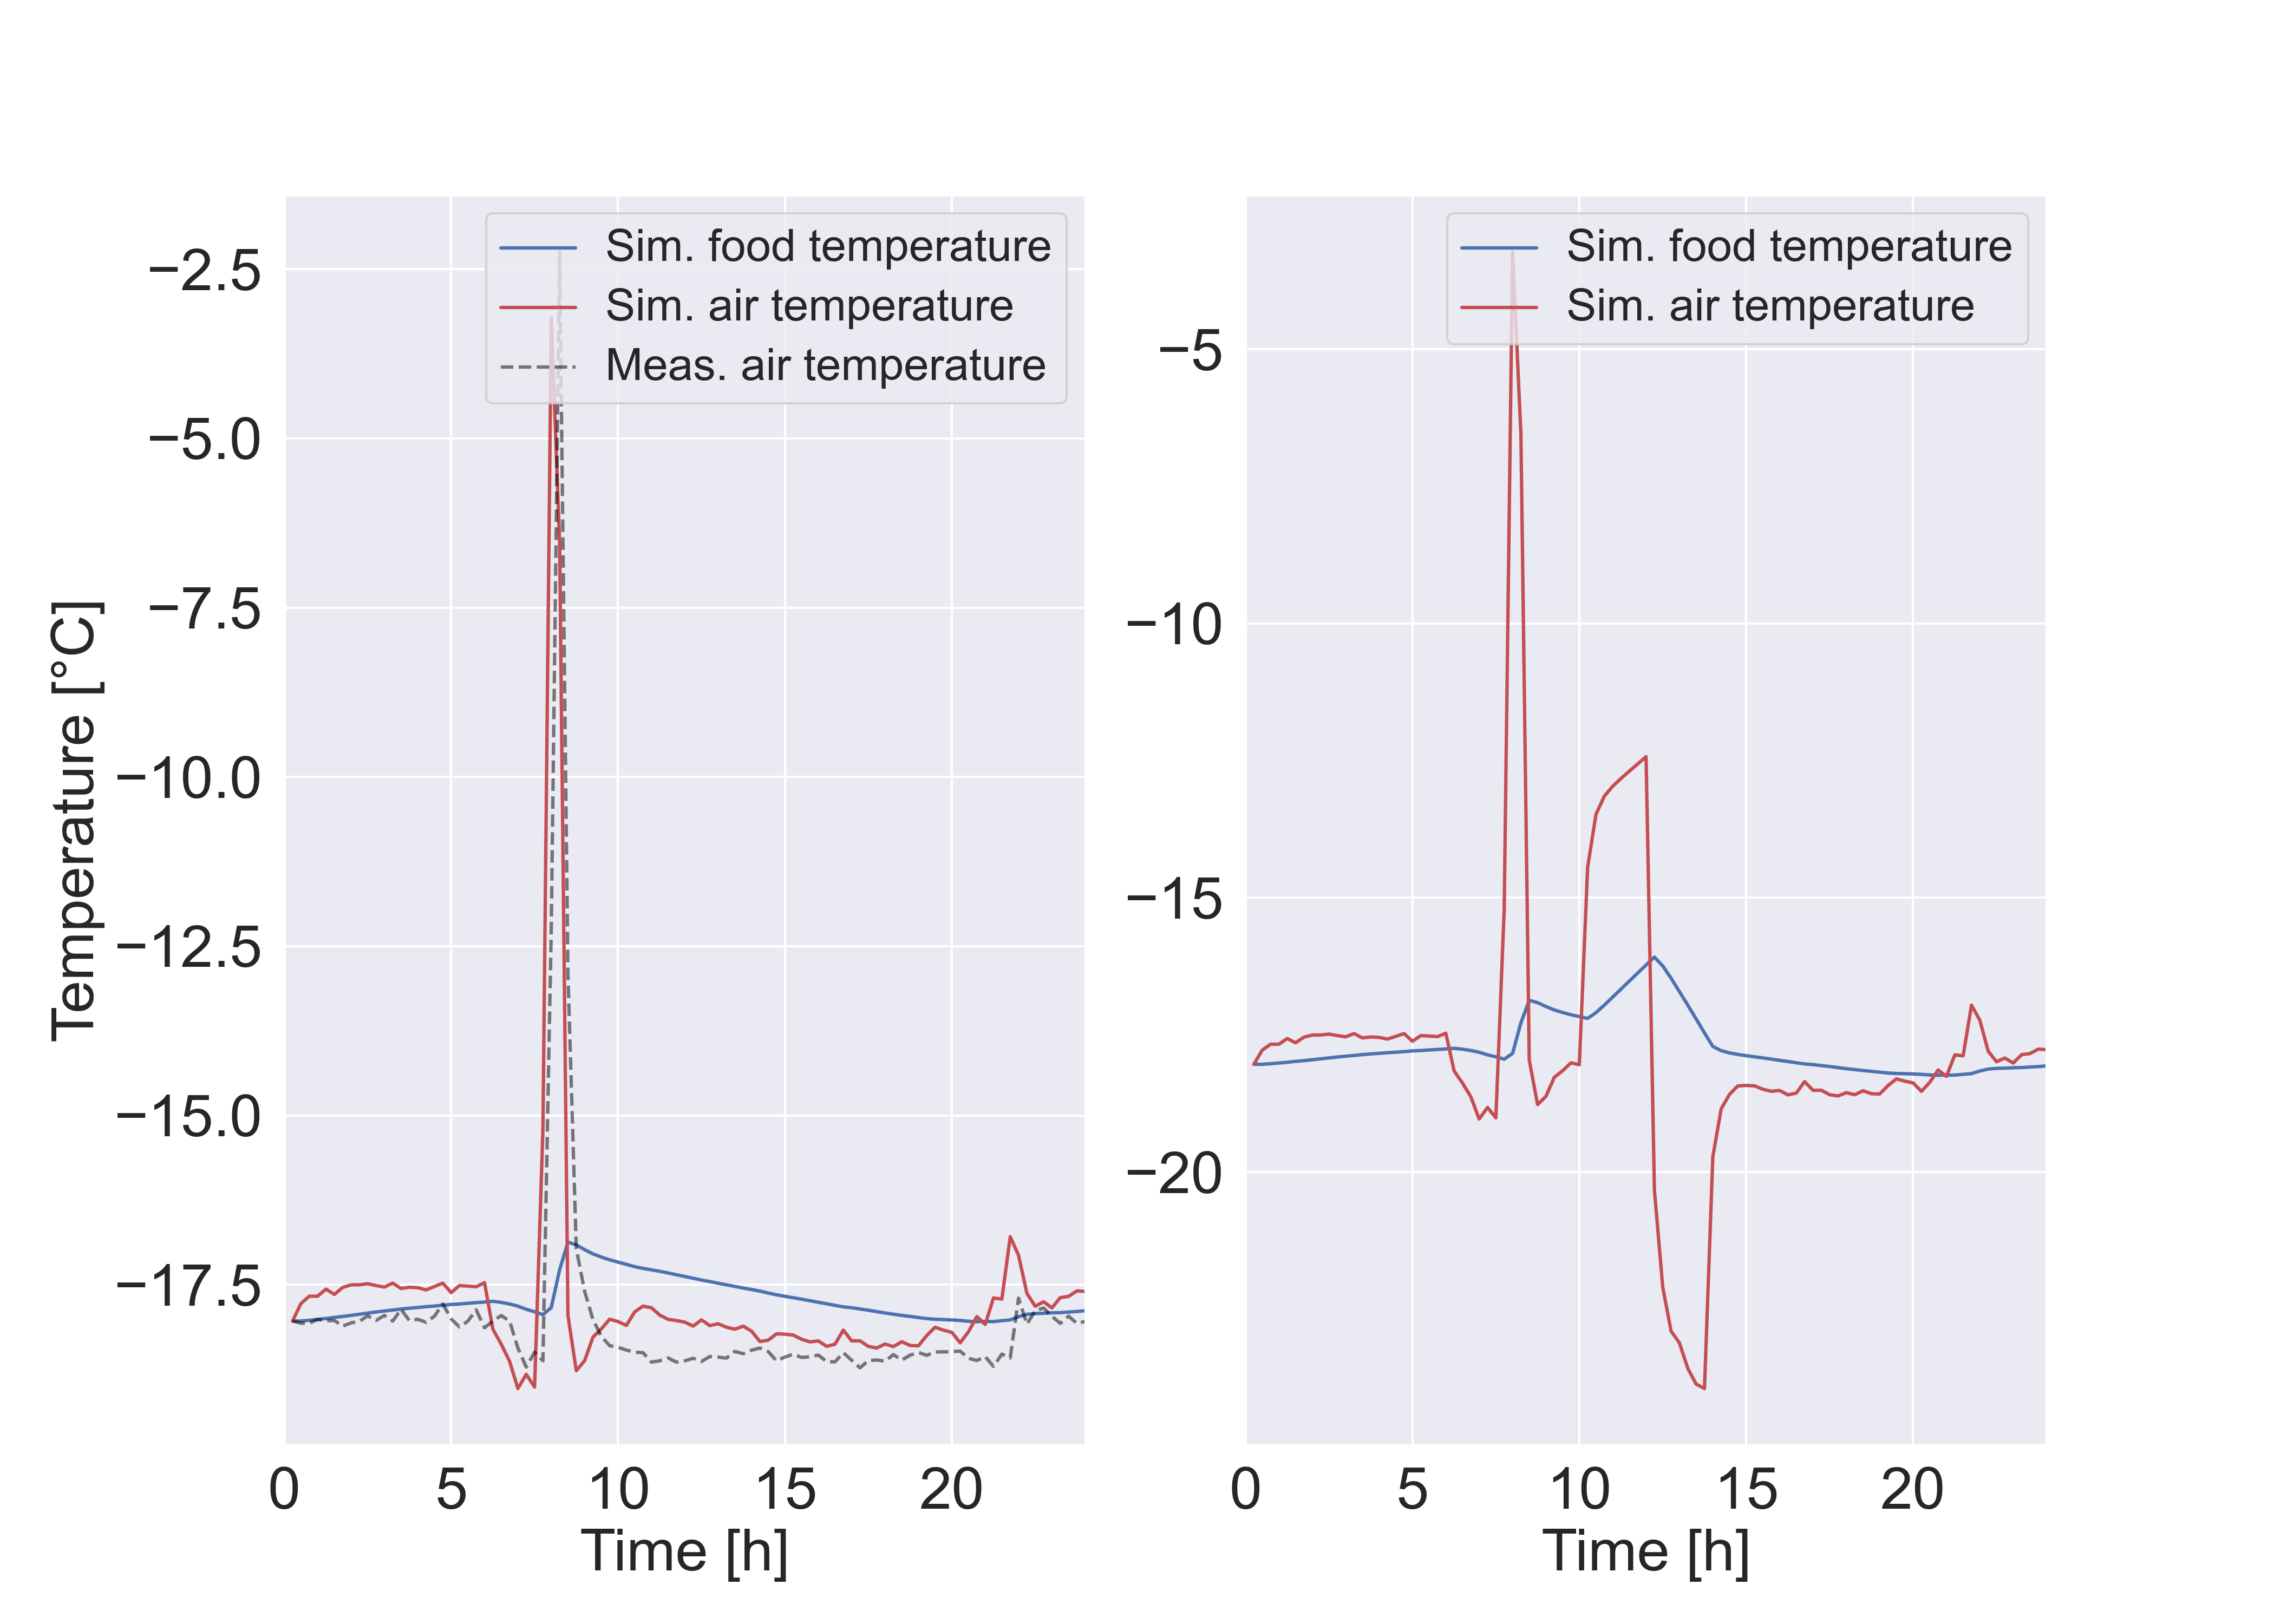
\includegraphics[width=\columnwidth]{../figures/2ndFreezerModelSimulation.png}
    \caption{ \textbf{Left}: Simulation of (\ref{eq:2ndFreezerStateSpace}) using the parameters in Table \ref{tab:parameter_estimates}. \textbf{Right}: Simulation where power is turned off for two hours with a subsequent rebound at the nominal power until the food temperature is back to its normal value.}
    \label{fig:2ndFreezerModelSimulation}
\end{figure}


\subsection{mFRR}\label{sec:mFRR}

Figure \ref{fig:timeline_mfrr} shows the timeline of the mFRR market in Denmark.\footnote{There is only a market for up-regulation.} One should note though, that BRPs can choose \textit{not} to bid in the reserve market and only bid real-time up and down-regulation. In this work, we consider the case where flexible demand delivers reservation through a BRP since payment is received for both reservation and activation. All prices considered are for DK2.\footnote{Denmark has two synchronous areas: DK1 (western part) and DK2 (eastern part).}

First, BRPs can bid reserve capacities in each hour, $p_{h}^{r,\uparrow}$ $\forall{h} \in \{1, \ldots 24 \}$, in the market for the next day, $D$. If accepted, they receive the reservation price, $\lambda_{h}^{r,\uparrow}$. This happens \textit{before} the day-ahead market clearing for which the BRPs buy energy for their expected demand, $P_{h}^{\text{Base}}$, at the spot price, $\lambda_{h}^{s}$. After that, a regulating power bid, $\lambda_{h}^{\text{bid}}$, must be submitted for each hour in $D$ where $p_{h}^{r,\uparrow} > 0$ \cite{energinet:Systemydelser}. In real-time, the reserves are activated if the following conditions hold, depending on the balancing price: $\{p_{h}^{r,\uparrow} > 0 \land \lambda_{h}^{\text{bid}} <  \lambda_{h}^{b} \land \lambda_{h}^{b} > \lambda_{h}^{s} \}$

% \begin{figure}[!t]
%     \centering
%     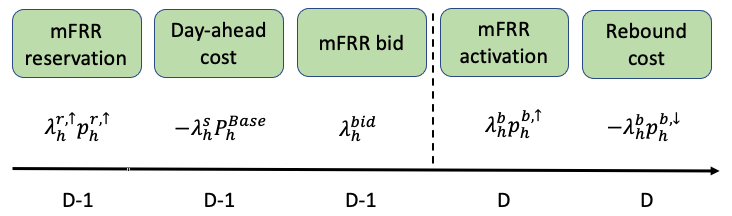
\includegraphics[width=\columnwidth]{../figures/timeline_mfrr.png}
%     \caption{Timeline of the Danish mFRR market.}
%     \label{fig:timeline_mfrr}
% \end{figure}


\begin{figure}[!t]
    \centering
    \includestandalone[width=\columnwidth]{../figures/timeline_mfrr_tikz}
    \caption{Timeline of the Danish mFRR market.}
    \label{fig:timeline_mfrr}
\end{figure}


If the conditions are met, the BRP receives the balancing price times their actual up-regulation, $p_{h}^{b,\uparrow}$. The BRP also incurs an additional cost due to any subsequent rebound. Furthermore, the BRP incurs a penalty, $s_{h} = \text{max}\{0, p_{h}^{r,\uparrow} - p_{h}^{b,\uparrow}$\}, if they don't deliver their promised reserve.

A suitable objective function for a BRP delivering mFRR up-regulation for one day is therefore:

\begin{align}\label{eq:mFRRObjective}
     % & \underbrace{C(\text{cost})}_{\text{mFRR}} = - \underbrace{\sum_{h=1}^{24} 
     &  - \underbrace{\sum_{h=1}^{24} \lambda^{s}_{h}P^{\text{Base}}_{h}}_{\textrm{Energy cost}} + \underbrace{\sum_{h=1}^{24}\lambda_{h}^{r} p^{r, \uparrow}_{h}}_{\textrm{Reservation payment}}  \notag \\ & \quad \quad + \underbrace{\sum_{h=1}^{24}  \lambda_{h}^{b} p^{b,\uparrow}_{h}}_{\textrm{Activation payment}} - \underbrace{\sum_{h=1}^{24}  \lambda_{h}^{b} p^{b,\downarrow}_{h}}_{\textrm{Rebound cost}} - \underbrace{ \sum_{h=1}^{24}  \lambda^{p}s_{h}}_{\textrm{Penalty cost}}
\end{align}


\subsection{Load shifting}

Another option for utilizing flexibility is to shift the load to a different time according to the spot prices which are known already 12-36 hours in advance. Then it is simply a matter of consuming in low-price hours and not in high-price hours.

For a TCL, there are additional constraints to how energy can be shifted also due to the rebound. First, there can be temperature constraints which will result in less energy being shifted. Second, the rebound must happen immediately after reducing power consumption (otherwise, the temperature deviation becomes too big for too long).

The savings from load shifting are directly proportional to the volume and price difference between the baseline load and shifted load as given by:

\begin{equation}\label{eq:load_shifting_savings}
    \sum_{h=1}^{24} \lambda^{s}_{h} p^{\text{Base}}_{h} - \lambda^{s}_{h} p^{\prime}_{h}
\end{equation}

where $p_{h}$ is the power profile during load shifting, $p^{\text{Base}}_{h}$ is the normal baseline power, and $\lambda^{s}_{h}$ is the spot price.

However, since the load shifting action only occurs \textit{after} the day-ahead market clearing (cf. Figure \ref{fig:timeline_mfrr}), the BRP has already bought $\lambda^{s}_{h} p^{\text{Base}}_{h}$ and any deviation results in an imbalance for the BRP. In this work, we look at the case where flexible demand acts selfishly and excludes the BRP from its load shifting action. Therefore, the objective function for the flexible demand is simply:

\begin{equation}\label{eq:LoadShiftingObjective}
    % \underbrace{C(\text{cost})}_{\text{load shifting}} = \sum_{h=1}^{24} \lambda_{h}^{s} p_{h}
    \sum_{h=1}^{24} \lambda_{h}^{s} p_{h}
\end{equation}
